\chapter{Convolutional Neural Network}
This chapter will break down the process needed to build, train and test a convolutional neural network with PyTorch. The PyTorch library comes with a lot of great tutorials that work well on the large datasets that they provide in order to load the data in bulk and train your neural network using GPUs to parallelise the process. However, the data that most remote sensing scientists have is not in tiles with one land use class per tile, but rather in extremely large images with lots of varied land use across the field of view. There are explanations on how to use this sort of varied data in order to train the model and this thesis aims to standardise this procedure for a binary classification. \newline
\textbf{http://cs231n.github.io/convolutional-networks/}
\paragraph{}
Convolutional Neural Networks or CNNs are similar to neural networks as they are made up of neurons with learnable weights and biases, just like random forests (RF) and support vector machine (SVM) learning. Each neuron receives an input, performs a dot product and then optionally follows with a non-linear function. Non-linear functions work like a sprinkler system in an agricultural field, which works to randomly spray the water in any direction so the whole field is targeted rather than just one straight line. 
\par Compared to regular neural networks, CNNs explicitly assume the inputs are images allowing certain properties to be encoded. Regular neural networks transform images through a series of hidden layers. Each layer is made up of neurons with each neuron connected to every neuron in the the previous layer but each neuron in one layer is not connect to any other neuron in the same layer. The last fully connected layer contains the class score for each pixel, indicating what class that class is most likely to belong to. Regular networks do not scale well to images that have multiple channels of information. For remote sensing, in most cases the imagery that is being looked at will have at least three layers of information, if not more. In a regular network, a image that is 256x256 pixels with three channels equates to 196,000 weights to calculate, for just one neuron. This requires lots of parameters and can lead to overfitting. \par
CNNs take advantage of the 3D volume of neurons so each neuron has height, width and depth dimensions where the depth corresponds to the number of bands in the image (Figure \ref{fig.convolve_data}). The network then works to convolve the information to allow the image to have a single vector class score that is arranged along the depth dimension. To summarise a CNN is a sequence of layers where each layer transforms one volume of activations to another through a differential function. For a generic CNN there is a convolutional layer, a pooling layer and a fully connected layer, these layers are then stacked to form a convolutional neural network.
\begin{figure}[H]
\centering
\begin{subfigure}{0.45\textwidth}
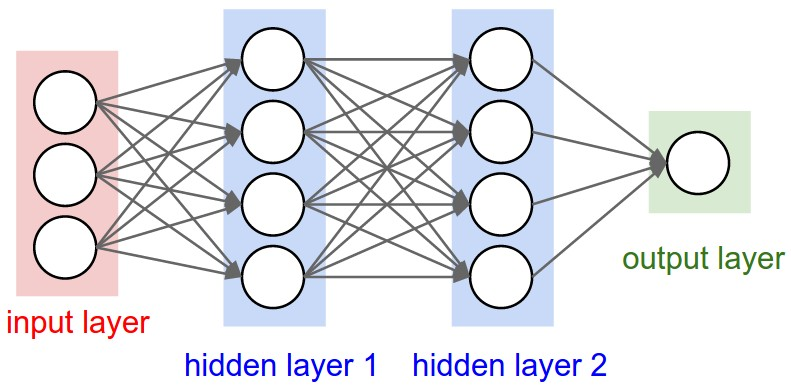
\includegraphics[width=\textwidth]{\dir/figs/convolve_data.jpeg}
\caption{}
\label{fig.convolve_data1}
\end{subfigure}%
\qquad
\begin{subfigure}{0.45\textwidth}
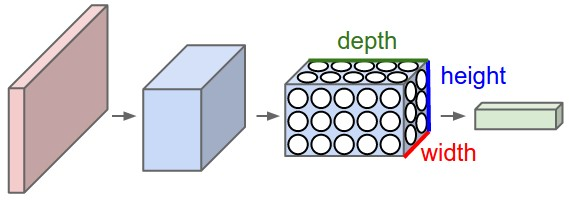
\includegraphics[width=\textwidth]{\dir/figs/convolve_data2.jpeg}
\caption{}
\label{fig.convolve_data2}
\end{subfigure}
\caption[Basic Convolutional Neural Network architecture]{\ref{fig.convolve_data1} Regular convolutional neural network. Circles represent neurons and neurons in each layer do not connect to one another. \ref{fig.convolve_data2} describes how the data is convolved, in each layer a 3D input is transformed into a 3D output of activations. The red input layers is the image, width and height are the dimensions of the image and the depth is the number of layers (3 bands for RGB).}
\label{fig.convolve_data}
\end{figure}

\begin{itemize}
    
    \item \hl{The \textbf{input} layer holds the raw pixel values, for this architecture that means 256x256x3 (width x height x number of bands).}
    \item \hl{The \textbf{convolutional (CONV)} layer computes the output of the neurons that are connected to local regions, each by computing a dot product between their weights and a small region they are connected to in the input volume.}
    \item \hl{The \textbf{RELU} layer applies an element-wise activation function, resulting in thresholding at 0, leaving the size unchanged.}
    \item \hl{The \textbf{pooling (POOL)} layer performs a downsampling along the width and height dimensions.}
    \item \hl{The \textbf{fully connected (FC)} layer computes the class score, as this architecture is looking at a binary classification, this is either of 2 classes, the object of interest or not.} 
\end{itemize}
\par
The network transforms the original image layer by layer from the original pixel values into the class scores. The CONV layer and the FC layers are functions of the activation in the input volume as well as the weights and biases of the neurons. The RELU and POOL layers always implement a fixed function. The parameters of CONV and FC are trained with gradient descent so that the class scores are consistent with the labels in the training image. In terms of our training data, the predicted class score is compared to the binary classification image to determine whether or not the network has accurately predicted the pixel value.
\par
\section{Construct the Neural Network}
Before beginning data loading and processing, a generic neural network is created to process the data. This is constructed in a way that can handle any datasets with a 3-channel RGB image with an associated binary mask. The next sub-section will outline architecture needed to do this and provide an in depth discussion.
\subsection{\textbf{CONV} layer}
The CONV layer is the core building block for the network. It consist of a set of learnable filters, each filter is spatially small but extends through the full depth of the input. Our network has been created with a filter of 4x4x3, where 4x4 represents the height and the width and 3 represents the depth of the input i.e. the number of channels or bands. This is shown in line 2 of listing \ref{lst.encoder}, where the kernel size is 4 and our in\_channel is 3. \par
As we move down through the network we pass or convolve each filter across the the width and height of the input volume, then compute the dot product between the entries of the filter and the input at any position. This produces a 2D activation map that gives the response of that filter at every spatial position. Intuitively the network learns filters that activate when they recognise some type of visual feature such as edges or blocks of colour in the first layer. This results in an entire set of filters in each CONV layer producing separate 2D activation maps that are then stacked together along the depth axis to produce the output volume.
\begin{lstlisting}[language=Python, caption = Encoder architecture, label={lst.encoder}]
class SegBlockEncoder(nn.Module):
    def __init__(self,in_channel,out_channel,kernel=4,
                stride=2,pad=1):
        super().__init__()
        self.model = nn.Sequential(
            nn.Conv2d(
                in_channel,out_channel,kernel,stride=stride,
                padding=pad,bias=False),
            nn.BatchNorm2d(out_channel),
            nn.ReLU(True)
        )

    def forward(self, x):
        y=self.model(x)
        return y
\end{lstlisting}
Firstly the data is fed into the encoder, the neural network takes in a set number of channels (i.e. 3 for an RGB image) and outputs a different number of channels.

When using images with multiple bands it is impractical to connect every neuron to all the neurons in the previous volume. Each neuron is therefore connected to a local region of the input volume as defined by the kernel size. Connections are then local within height and width but always fully connected along the depth depth of the input volume (Figure \ref{fig.conv_layer}). 
\begin{figure}[H]
    \centering
    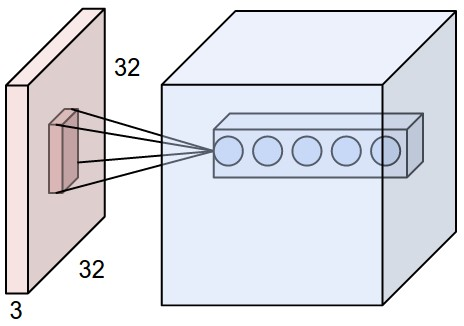
\includegraphics[width=0.5\textwidth]{\dir/figs/depthcol.jpeg}
    \caption[CONV Layer]{An example of the red input volume and an example of the neurons in the first convolutional layer. Each neuron in the layer is only connected to a local region in the input layer spatially, but to the full depth which in this case is 5 neurons.}
    \label{fig.conv_layer}
\end{figure}
Neurons in the output layer are controlled by the depth, stride and padding. 
\begin{enumerate}
    \item Depth of the output volume corresponds to the number of filters used to look for something in the input. For example to look for edges or colours. This is adjusted manually when fine-tuning the network in order to optimise the results.
    \item Stride for our case equals two and it defines how much the filter steps by as it moves over the image. Using two reduces the size of the output image.
    \item Padding controls the number of layers of zeroes around the input volume. 
\end{enumerate}
\subsection{Batch Normalisation}
Batch normalisation is a function that is used to correct for the effect of changing inputs as the network moves from layer to layer. \citet{ioffe15} were the first to recognise the affect that internal covariate shift had on deep learning. Within a single training set, the affect of internal covariate shift is not that significant but if the network is intended to predict values in another area, the effect can result in a very inaccurate model. Covariate shift is a result of bias in the dataset and a more in depth look and examples of the effect can be found in \citet{smola11}. By reducing the internal covariate shift, learning rates can be higher improving the time needed to achieve highly accurate models. The paper by \citet{ioffe15} claims that by using a batch normalisation function the validation error of the ImageNet classification can be dropped to below 5\% and this is better than the error expected from human raters. The normalisation occurs on the batch and is separated from the optimiser and gradient descent. This means that the parameters are adjusted independently of the optimiser and allows for faster learning rates. 
\par
\hl{Useful explanation of batch norm: https://kratzert.github.io/2016/02/12/understanding-the-gradient-flow-through-the-batch-normalization-layer.html}
\subsection{Activation Layer}
There are many different types of activation functions that can be used with CNNs. Some of functions are better suited to different applications. ReLU(Rectified Linear Unit) is the most reliable and can be used as a good approximation for all applications. \par
Activation functions introduce non-linear properties on the network and convert an input signal to an output one. They sum the product of the inputs and their corresponding weights and apply the function to get the output and feed it as an input for the next layer. Without an activation function the output would be a linear function. These are limited in their complexity and cannot learn complex functional maps from the data. A neural network without an activation function is simply a linear regression model. Activation functions allow the user to represent non-linear arbitrary functional mappings between inputs and outputs. \par
\begin{figure}[H]
    \centering
    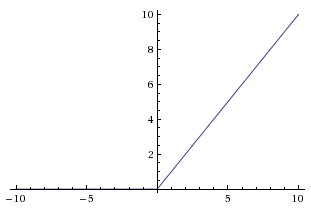
\includegraphics[width=0.5\textwidth]{\dir/figs/relu.jpeg}
    \caption{ReLu function.}
    \label{fig.relu}
\end{figure}
ReLU corrects a value to be 0 when $<$ 0 and then linear with slope of 1 when x $>$ 0. Figure \ref{fig.relu} shows the function in graphical form. \citet{krizhevsky17} shows the ReLU functions to be 6 times faster than Tanh. 
\subsection{Pool Layer}

\subsection{Fully Connected}

\subsection{Decoder}

\subsection{Neural Network}
\section{Data Processing and and Loading}
For the a user wanting to load and train a network they first need to prepare their data so that it is in the right format to be read by the network. In remote sensing, a user may commonly have one image of 30,000x30,000 pixels if they have a 10x10km tile at ~30cm resolution. This needs to be transformed and reduced in size to train a network. The networks would not be trained very well if just one image was fed in, especially at the extreme size of 30,000x30,000 pixels. The first step of the process is to transform and crop this data so that only a small section of the image is being fed into the network. The transform class used for this function can be found below (Listing \ref{lst.transform}).
\subsection{Convert image data to correct format}
In order for the image data to work within PyTorch it needs to be in the PIL format. The training and test dataset used for the creating of the workflow were in .tif format and so no conversion was needed. If the data type the user intended to use was not in the PIL format, a conversion would be necessary.
\subsection{Transform the Data}
Transforms on the data need to be performed on both the image layer and thr binary mask in tandem. In order to do this a custom transform class was written to ensure that these transformed were mirrored and the two layers of information remained paired and undistorted.
The arguments for the transform class are lists of all the users image and associated and binary mask files. The user can remove the comment at Listing \ref{lst.transform} line 16-19 if their training data is not all of the same dimensions. The class then proceeds to crop, horizontally flip, vertically flip, and eventually transform the data arrays into PyTorch tensors that can be fed into the neural network. \par 
 \begin{lstlisting}[language=Python, caption = Transform Class, label={lst.transform}]
class BuildingsDataset(Dataset):
    """INRIA buildings dataset"""
    
    def __init__(self,images_dir,gt_dir,train=True):
        """
        Args:
        images_dir = path to the satellite images
        gt_dir = path to the binary mask
        """
        self.image_paths = images_dir
        self.target_paths = gt_dir
        self.train=train
        
    def transform(self, image, mask):
        # Resize
#         resize = transforms.Resize(size=(5000, 5000))
#         image = resize(image)
#         mask = resize(mask)

        # Random crop
        i, j, h, w = transforms.RandomCrop.get_params(
            image, output_size=(256, 256))
        image = TF.crop(image, i, j, h, w)
        mask = TF.crop(mask, i, j, h, w)
        
        # Random horizontal flipping
        if random.random() > 0.5:
            image = TF.hflip(image)
            mask = TF.hflip(mask)
            
        # Random vertical flipping
        if random.random() > 0.5:
            image = TF.vflip(image)
            mask = TF.vflip(mask)
            
        # Transform to tensor
        image = TF.to_tensor(image)
        mask = TF.to_tensor(mask)
        mask = torch.cat([(mask==0).float(),(mask==1).float()],dim=0)
        return image, mask
        
    def __getitem__(self, index):
        image = Image.open(self.image_paths[index])
        mask = Image.open(self.target_paths[index])
        x, y = self.transform(image, mask)
        return x, y
        
    def __len__(self):
        return len(self.image_paths)
\end{lstlisting}
There is an additional transformation that is applied to the mask. The binary mask comes as one layer where the minimum value corresponds to what is not of interest and the max value corresponds to where there is something of interest (Listing \ref{lst.transform} line 39). The transform splits this single layer into two layers. In the first layer, where the value was minimum it now shows as max and the opposite is the case for the second layer (Figure \ref{fig.binary_mask}) . This is so that when a class probability is determined by the network this can then predict which layer the pixel is most likely to belong to. In essence this process has transformed the data into two classes rather than just one.
\begin{figure}[H]
    \centering
    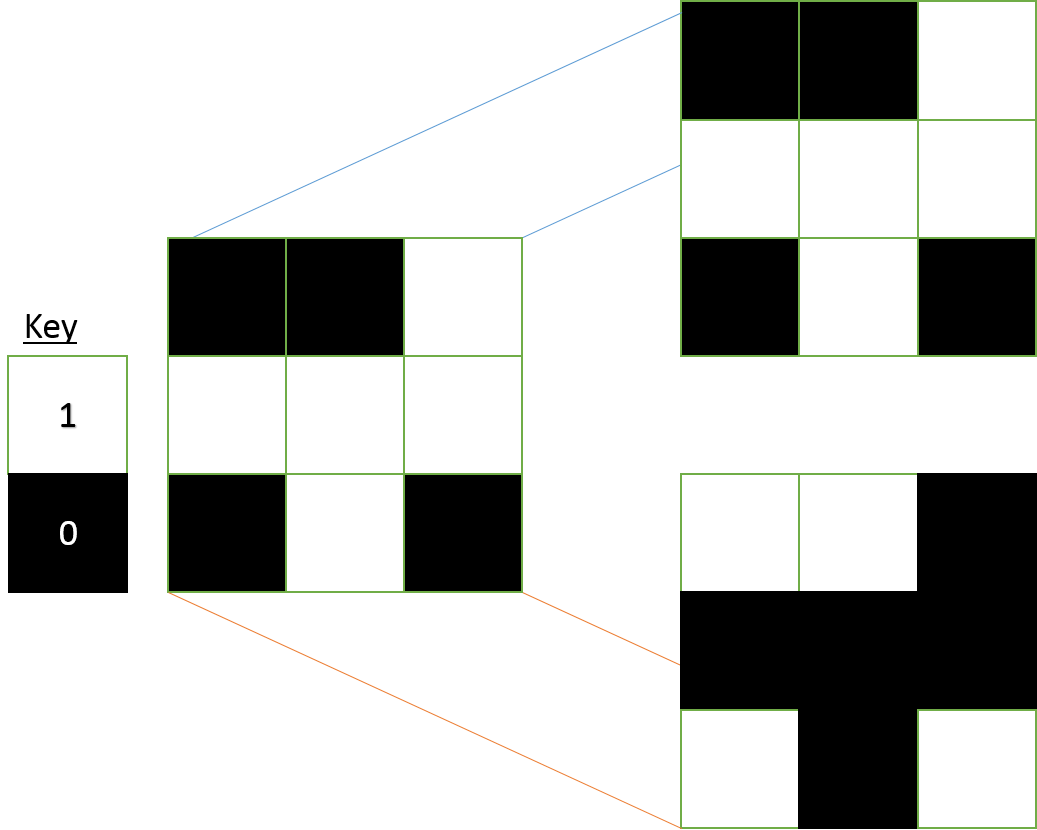
\includegraphics[width=0.5\textwidth]{\dir/figs/binary_mask.png}
    \caption[Binary Mask]{The grid on the left shows the original binary classification, where white shows the class of interest and the black shows nothing. On the right, the upper grid shows white where the original image showed white. On the right the lower grid shows white where the original grid showed black.}
    \label{fig.binary_mask}
\end{figure}
The transform function outputs an array with two item, where the first item is the image as a tensor and the second item is the associated binary mask as a tensor. This datatype is then ready to be loaded directly into the neural network.
\subsection{Load the Data}
PyTorch has a in-build dataloader class that is used to batch and load the data. It can even be used to load the data using GPU if the user had access to one. The data needs to be prepared in a certain way in order to be loaded through this class. The transform class prepares the data into this specific format so it can be bulk loaded into the network. The dataloader then batches, shuffles and loads the data, either in parallel or not, into the neural network for training. Figure \ref{fig.dataloader} shows how the data looks as it is being fed into the CNN. There is a randomly cropped RGB image with an associated binary mask, which is made up of two layers, the first layer being displayed as 1 where the class is, the second showing 1 where the class is not. 
\begin{figure}
    \centering
    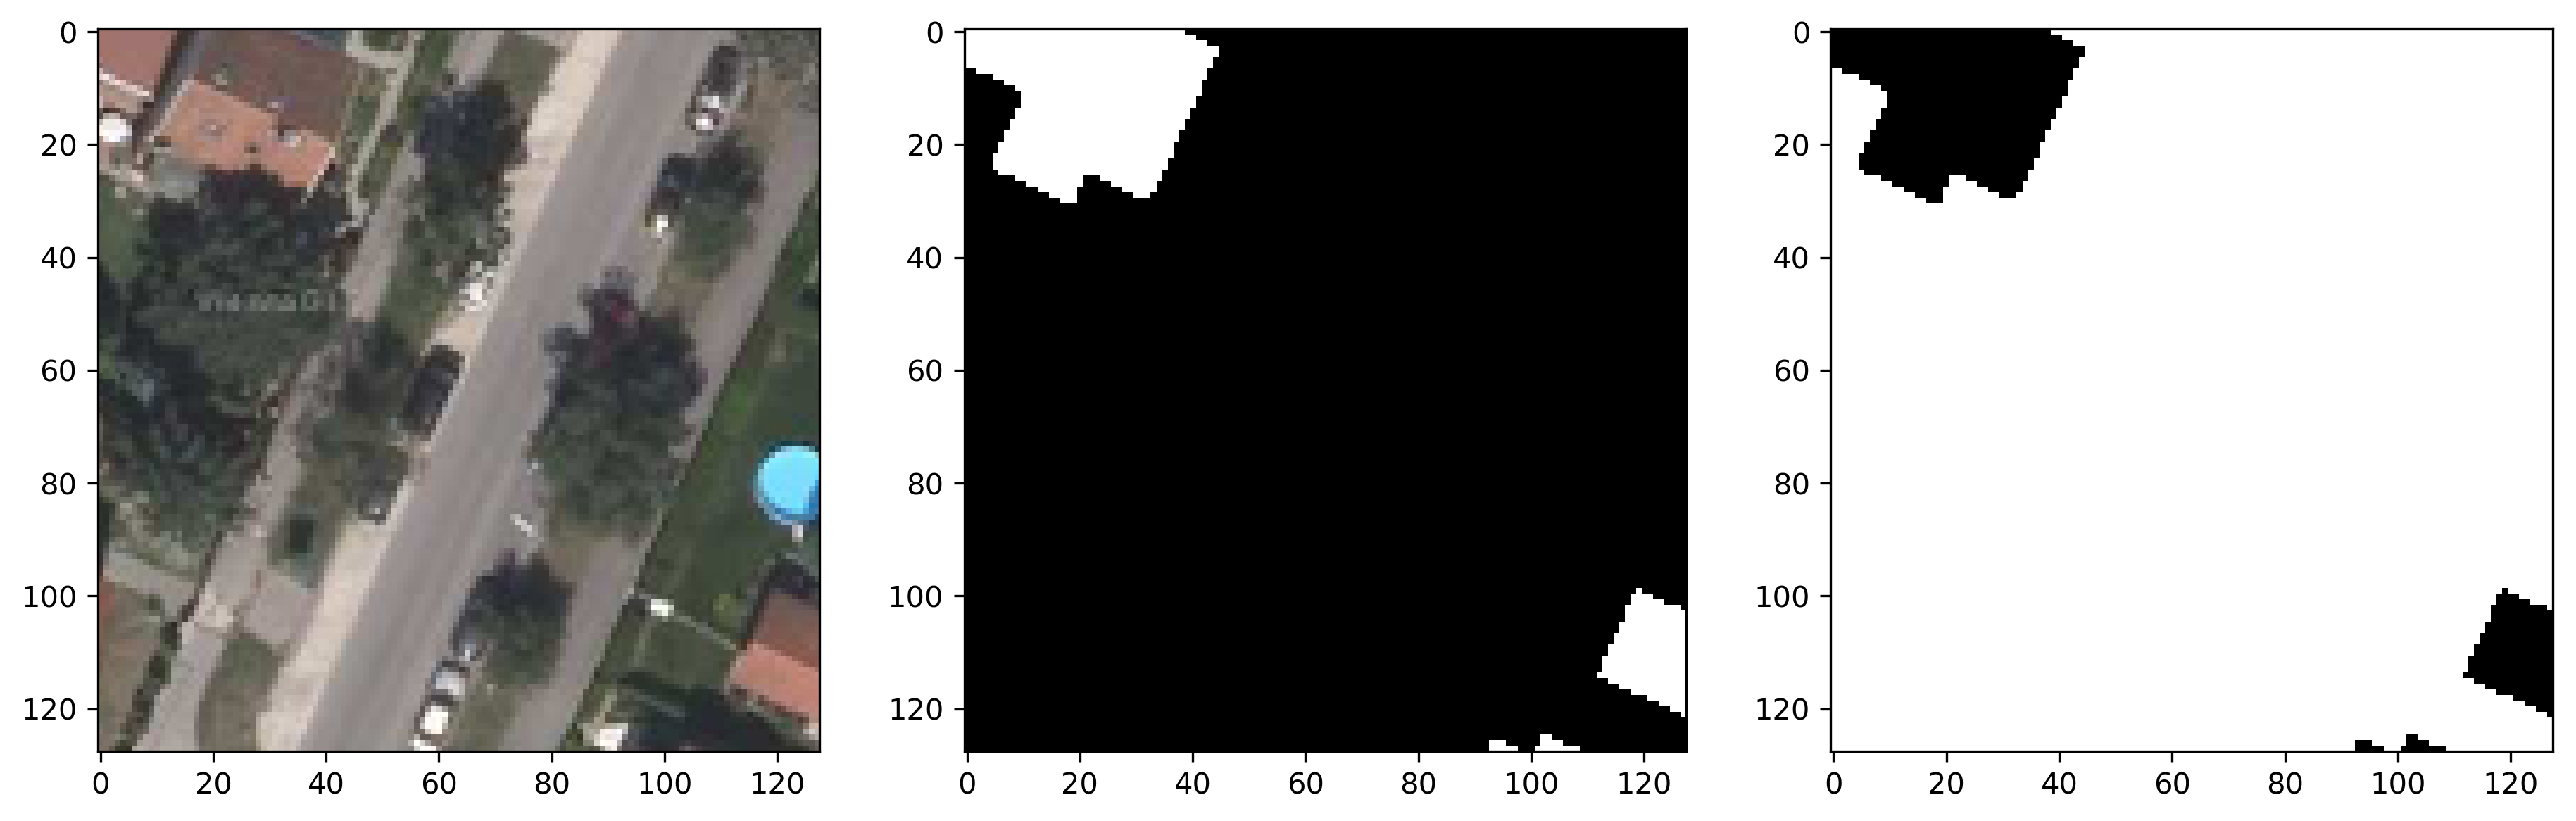
\includegraphics[width=1\textwidth]{\dir/figs/example_dataloader.png}
    \caption[Example of how the dataloader handles the data]{Example of how the dataloader handles the data. This image shows a random 128x128 crop from a random tile within the dataset. The dataloader constructs these paired images into a stack that can be defined by the user and optimised to reduce processing times. On the left is the RGB image, the middle shows as positive where there are buildings and the left shows as positive where buildings are not.}
    \label{fig.dataloader}
\end{figure}
\section{Training the Network}
Once the network has been constructed the user needs to tune the hyperparameters in order to get the best loss and learning rate from their network in the shortest possible time. This is the most time consuming and frustrating part of the process as there are many different parts of the network that can be adjusted to produce different results. The three hyperparameters that need to be adjusted are as follows:
\begin{itemize}
    \item The number of depth of the convolutional layer
    \item The batch size
    \item The learning rate for the optimiser.
\end{itemize}
These will be discussed further in the next section.
\subsection{Convolution Depth}
The convolution depth determines the architecture of the neural network. The user has to decide what value to start with as this dictates how deep the output of the final convolutional layer will be.
\subsection{Batch Size}
\subsection{Learning Rate and Optimizer}


\section{Testing the Network}